% 图 5.18 MnO 磁结构：双 fcc 胞、(111) 面自旋黑白交替
\documentclass[tikz,border=5pt]{standalone}
\usetikzlibrary{arrows.meta,calc}
\usepackage{amsmath}
\usepackage{bm}
\usepackage{fontspec}
\setmainfont{Times New Roman}
\begin{document}
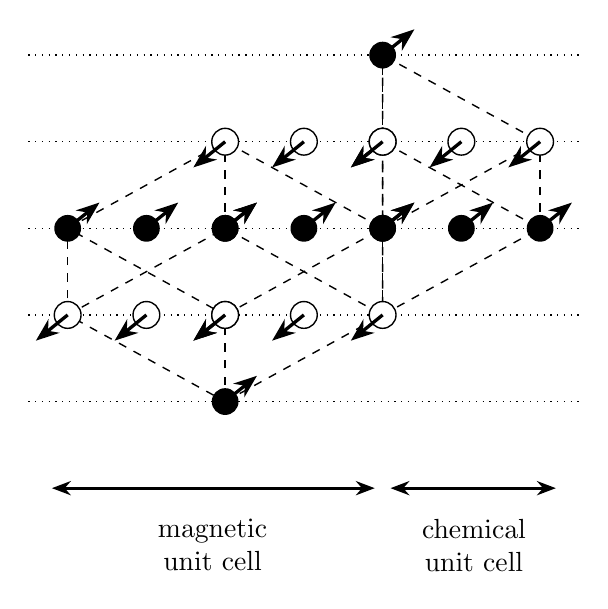
\begin{tikzpicture}[line width=0.8pt,>=Stealth]
\begin{scope}[scale=2.0]
  % (111) plane traces
  \foreach \s in {0,...,4}{
    \draw[dotted,line width=0.45] (-1.25,{0.55*\s}) -- (2.25,{0.55*\s});}
  % two fcc cells, dashed edges
  \draw[dashed,line width=0.5] (0,0) -- (1,0.55) -- (0,1.1) -- (-1,0.55) -- cycle;
  \draw[dashed,line width=0.5] (0,0.55) -- (1,1.1) -- (0,1.65) -- (-1,1.1) -- cycle;
  \draw[dashed,line width=0.5] (0,0) -- (0,0.55) (-1,0.55) -- (-1,1.1)
        (1,0.55) -- (1,1.1) (0,1.1) -- (0,1.65);
  \draw[dashed,line width=0.5] (1,0.55) -- (2,1.1) -- (1,1.65) -- cycle;
  \draw[dashed,line width=0.5] (1,1.1) -- (2,1.65) -- (1,2.2) -- cycle;
  \draw[dashed,line width=0.5] (2,1.1) -- (2,1.65) (1,1.65) -- (1,2.2);
  % atoms: 12 corners + 11 face centres (sign by parity of x+y+z)
  \newcommand\atom[4]{{%
    \coordinate (A) at ({#1-#2},{0.55*(#1+#2+#3)});
    \ifnum#4>0 \fill (A) circle (0.085); \else
      \fill[white,draw=black,line width=0.5] (A) circle (0.085); \fi
    \draw[->,line width=1.2] (A) -- ++(\ifnum#4>0 39\else 219\fi:0.26);}}
  \atom{0}{0}{0}{1}   \atom{0}{0}{1}{-1}  \atom{0}{1}{0}{-1}  \atom{0}{1}{1}{1}
  \atom{1}{0}{0}{-1}  \atom{1}{0}{1}{1}   \atom{1}{1}{0}{1}   \atom{1}{1}{1}{-1}
  \atom{2}{0}{0}{1}   \atom{2}{0}{1}{-1}  \atom{2}{1}{0}{-1}  \atom{2}{1}{1}{1}
  \atom{1}{0.5}{0.5}{1} \atom{0}{0.5}{0.5}{-1} \atom{2}{0.5}{0.5}{-1}
  \atom{0.5}{0.5}{0}{-1} \atom{0.5}{0.5}{1}{1}
  \atom{1.5}{0.5}{0}{1}  \atom{1.5}{0.5}{1}{-1}
  \atom{0.5}{0}{0.5}{-1} \atom{0.5}{1}{0.5}{1}
  \atom{1.5}{0}{0.5}{1}  \atom{1.5}{1}{0.5}{-1}
  % cell spans
  \draw[{Stealth[length=2.4mm]}-{Stealth[length=2.4mm]},line width=1.0]
    (-1.1,-0.55) -- (0.95,-0.55);
  \draw[{Stealth[length=2.4mm]}-{Stealth[length=2.4mm]},line width=1.0]
    (1.05,-0.55) -- (2.1,-0.55);
  \node[align=center,anchor=north] at (-0.08,-0.68) {magnetic\\unit cell};
  \node[align=center,anchor=north] at (1.58,-0.68) {chemical\\unit cell};
\end{scope}
\end{tikzpicture}
\end{document}
